\documentclass[aspectratio=169,12pt,t]{beamer}

% --- Theme: Metropolis (modern, clean) ---
\usetheme[progressbar=frametitle,numbering=fraction,block=fill]{metropolis}

% --- Fira Sans font (install texlive-fonts-extra if missing) ---
\IfFileExists{FiraSans.sty}{\usepackage[sfdefault]{FiraSans}}{}

% --- Light background with warm accent ---
\definecolor{mDarkTeal}{RGB}{35,55,59}
\definecolor{mLightBrown}{RGB}{235,228,216}
\definecolor{mAccent}{RGB}{140,70,20}

\setbeamercolor{normal text}{fg=mDarkTeal,bg=white}
\setbeamercolor{alerted text}{fg=mAccent}
\setbeamercolor{frametitle}{bg=mDarkTeal,fg=white}
\setbeamercolor{progress bar}{fg=mAccent,bg=mLightBrown}
\setbeamercolor{title separator}{fg=mAccent}
\setbeamercolor{progress bar in head/foot}{fg=mAccent,bg=mLightBrown}
\setbeamercolor{progress bar in section page}{fg=mAccent,bg=mLightBrown}

% --- Packages ---
\usepackage[utf8]{inputenc}
\usepackage{amsmath,amssymb,amsthm}
\usepackage{mathrsfs}
\usepackage{tikz}
\usetikzlibrary{arrows.meta,positioning,calc,decorations.pathreplacing,shapes,patterns}
\usepackage{pgfplots}
\pgfplotsset{compat=1.18}

% --- Custom colors for content types ---
\definecolor{defcolor}{RGB}{25,85,120}
\definecolor{thmcolor}{RGB}{140,35,35}
\definecolor{proofcolor}{RGB}{35,100,50}
\definecolor{excolor}{RGB}{140,75,10}
\definecolor{remcolor}{RGB}{90,90,90}

% --- Beamer blocks for mathematical content types ---
\newenvironment{defblock}[1]{%
  \setbeamercolor{block title}{bg=defcolor,fg=white}%
  \setbeamercolor{block body}{bg=defcolor!5}%
  \begin{block}{#1}}{\end{block}}

\newenvironment{thmblock}[1]{%
  \setbeamercolor{block title}{bg=thmcolor,fg=white}%
  \setbeamercolor{block body}{bg=thmcolor!5}%
  \begin{block}{#1}}{\end{block}}

\newenvironment{proofblock}[1]{%
  \setbeamercolor{block title}{bg=proofcolor,fg=white}%
  \setbeamercolor{block body}{bg=proofcolor!5}%
  \begin{block}{#1}}{\end{block}}

\newenvironment{exblock}[1]{%
  \setbeamercolor{block title}{bg=excolor,fg=white}%
  \setbeamercolor{block body}{bg=excolor!5}%
  \begin{block}{#1}}{\end{block}}

\newenvironment{remblock}[1]{%
  \setbeamercolor{block title}{bg=remcolor,fg=white}%
  \setbeamercolor{block body}{bg=remcolor!5}%
  \begin{block}{#1}}{\end{block}}

% --- Metadata ---
\title{Chapter 3: Numerical Sequences and Series}
\subtitle{Section: Convergent Sequences}
\author{Based on Walter Rudin's \emph{Principles of Mathematical Analysis}}
\date{}

\begin{document}

% =============================================================================
% TITLE AND OUTLINE
% =============================================================================
{
\usebackgroundtemplate{%
  
\includegraphics[width=\paperwidth,height=\paperheight,keepaspectratio=false]{slide_background_01.png}%
}
\begin{frame}[plain]
  \titlepage
  \note{
    Welcome to Chapter 3 of Principles of Mathematical Analysis. This
    chapter is where analysis really begins. The central idea is that of
    a limit, and the first place we meet limits is in the study of
    sequences. In this opening section we define what it means for a
    sequence in a metric space to converge to a point, work through five
    concrete examples, and then establish the basic theorems that tell us
    how convergence interacts with neighborhoods, uniqueness, boundedness,
    limit points, and the algebraic operations of addition, multiplication,
    and division. Let us begin.
  }
\end{frame}
}

% =============================================================================
{
\usebackgroundtemplate{%
  
\includegraphics[width=\paperwidth,height=\paperheight,keepaspectratio=false]{slide_background_01.png}%
}
\begin{frame}{Outline}
  \tableofcontents
  \note{
    Here is the plan. We start with the formal definition of a convergent
    sequence and look at five examples that cover the main behaviors. We
    then prove Theorem 3.2, which collects four fundamental properties of
    convergent sequences. After that we turn to arithmetic: Theorem 3.3
    shows that limits respect sums, products, and reciprocals for complex
    sequences, and Theorem 3.4 extends these results to sequences in
    "R" to the "k". We close with a summary of the main takeaways.
  }
\end{frame}
}

% =============================================================================
% MOTIVATION
% =============================================================================

% --- Build 1/3 ---
\begin{frame}{Why This Section Matters}
  \begin{itemize}
    \item The whole of analysis is built on one idea: the \alert{limit}
  \end{itemize}

  \note{
    The whole of analysis is built on a single idea, the notion of a
    limit. Derivatives are limits of difference quotients, integrals are
    limits of Riemann sums, continuity is a statement about limits of
    function values, and series are limits of partial sums. Every major
    tool in this book ultimately traces back to this one concept.
  }
\end{frame}

% --- Build 2/3 ---
\begin{frame}{Why This Section Matters}
  \begin{itemize}
    \item The whole of analysis is built on one idea: the \alert{limit}
    \item The simplest limits live in \alert{sequences}: $p_1, p_2, p_3, \dots$
  \end{itemize}

  \note{
    The simplest setting in which limits appear is the setting of
    sequences. A sequence is just an infinite list of points indexed by
    the natural numbers: "p" sub 1, "p" sub 2, "p" sub 3, and so on. We
    want to understand when such a list of points has a well-defined
    destination, a point the list is getting arbitrarily close to.
  }
\end{frame}

% --- Build 3/3 ---
\begin{frame}{Why This Section Matters}
  \begin{itemize}
    \item The whole of analysis is built on one idea: the \alert{limit}
    \item The simplest limits live in \alert{sequences}: $p_1, p_2, p_3, \dots$
    \item Metric spaces give us the general framework: $d(p_n, p) \to 0$
  \end{itemize}

  \note{
    We work in the general setting of a metric space, because the basic
    facts about convergence are equally clean there as in the real line.
    Having a distance function "d" is all we need. Convergence then has
    a very compact expression: the distance from the "n"-th term to the
    limit goes to zero. Let us make this precise.
  }
\end{frame}

% =============================================================================
\section{Definition and Examples}
% =============================================================================

% --- Def 3.1: Build 1/2 ---
\begin{frame}{Definition 3.1: Convergent Sequence}
  \begin{defblock}{Definition 3.1 --- Convergence}
    A sequence $\{p_n\}$ in a metric space $X$ \alert{converges} if there
    is a point $p \in X$ such that:
    \[
      \forall\,\varepsilon > 0 \;\;\exists\, N \in \mathbb{N} \;\; \text{with} \;\;
      n \geq N \;\Longrightarrow\; d(p_n, p) < \varepsilon.
    \]
  \end{defblock}

  \note{
    Here is the official definition. A sequence "p" sub "n" in a metric
    space "X" converges if there is a target point "p" in "X" with the
    following property. For every positive tolerance epsilon, we can find
    an index "N" so that, from "N" onward, every term of the sequence
    lies within distance epsilon of "p". The tolerance epsilon is arbitrary:
    no matter how small we demand the distance to be, eventually the
    sequence gets that close and stays that close. The index "N" in general
    depends on epsilon, and it may be very large for very small epsilon.
  }
\end{frame}

% --- Def 3.1: Build 2/2 ---
\begin{frame}{Definition 3.1: Notation and Terminology}
  \begin{defblock}{Definition 3.1 --- Convergence}
    $\forall\,\varepsilon > 0 \;\;\exists\, N$ with $n \geq N \Longrightarrow d(p_n, p) < \varepsilon$.
  \end{defblock}

  \vspace{0.3em}
  \textbf{Notation and terminology:}
  \begin{itemize}
    \item $p$ is the \alert{limit} of $\{p_n\}$; write $p_n \to p$ or $\displaystyle\lim_{n\to\infty} p_n = p$.
    \item If no such $p$ exists, $\{p_n\}$ \alert{diverges}.
  \end{itemize}

  \note{
    With the definition in hand, we introduce some standard language.
    The point "p" is called the limit of the sequence, and we write
    either an arrow notation, "p" sub "n" arrow "p", or the usual limit
    notation, the limit as "n" goes to infinity of "p" sub "n" equals
    "p". If no such point exists inside the metric space "X", the
    sequence is said to diverge. We will soon see that when a limit
    exists it is unique, which justifies calling it the limit rather
    than a limit.
  }
\end{frame}

% --- Picture of convergence ---
\begin{frame}{Picture: What Convergence Looks Like}
  \begin{center}
  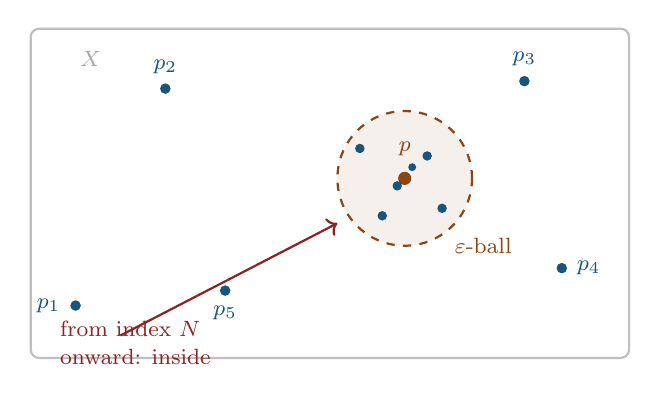
\begin{tikzpicture}[scale=0.95]
    % Outer ambient box (suggests metric space X)
    \draw[gray!50, thick, rounded corners=3pt] (-3.8,-2.2) rectangle (4.2,2.2);
    \node[gray!70] at (-3.0,1.8) {\footnotesize $X$};
    % epsilon-ball (disk) around p
    \fill[mAccent!8] (1.2,0.2) circle (0.9);
    \draw[mAccent, dashed, thick] (1.2,0.2) circle (0.9);
    \node[mAccent] at (2.25,-0.7) {\footnotesize $\varepsilon$-ball};
    % Limit point p
    \fill[mAccent] (1.2,0.2) circle (2.5pt);
    \node[mAccent, above=2pt] at (1.2,0.3) {\footnotesize $p$};
    % Sequence points spiraling inward
    \fill[defcolor] (-3.2,-1.5) circle (2pt) node[left=2pt]{\footnotesize $p_1$};
    \fill[defcolor] (-2.0,1.4) circle (2pt) node[above=2pt]{\footnotesize $p_2$};
    \fill[defcolor] (2.8,1.5) circle (2pt) node[above=2pt]{\footnotesize $p_3$};
    \fill[defcolor] (3.3,-1.0) circle (2pt) node[right=2pt]{\footnotesize $p_4$};
    \fill[defcolor] (-1.2,-1.3) circle (2pt) node[below=2pt]{\footnotesize $p_5$};
    % Inside the ball: later terms
    \fill[defcolor] (0.6,0.6) circle (1.8pt);
    \fill[defcolor] (1.7,-0.2) circle (1.8pt);
    \fill[defcolor] (0.9,-0.3) circle (1.8pt);
    \fill[defcolor] (1.5,0.5) circle (1.8pt);
    \fill[defcolor] (1.1,0.1) circle (1.8pt);
    \fill[defcolor] (1.3,0.35) circle (1.5pt);
    % Arrow + label for "index N onward"
    \draw[thmcolor, thick, ->] (-2.6,-1.9) -- (0.3,-0.4);
    \node[thmcolor, align=left] at (-2.4,-2.0) {\footnotesize from index $N$\\[-2pt]\footnotesize onward: inside};
  \end{tikzpicture}
  \end{center}

  \vspace{0.3em}
  No matter how small the $\varepsilon$-ball around $p$, \alert{eventually} every term lies inside.

  \note{
    Here is the geometric picture, drawn in a general metric space "X".
    The orange dot in the middle is the limit point "p", surrounded by
    a dashed circle: the epsilon-ball of all points within distance
    epsilon of "p". The blue dots are the terms of the sequence. Early
    terms scatter throughout the space, but from some index "N" onward,
    indicated by the arrow, every term lies inside the epsilon-ball.
    The crucial feature is that this is true for every epsilon: if we
    shrink the ball, the threshold "N" may grow, but eventually the
    sequence still lands inside.
  }
\end{frame}

% --- Dependence on X: Build 1/2 ---
\begin{frame}{Convergence Depends on the Space $X$}
  \begin{remblock}{Observation}
    Convergence depends on \alert{both} $\{p_n\}$ \alert{and} the ambient metric space $X$.
  \end{remblock}

  \vspace{0.5em}
  \textbf{Example:} $s_n = 1/n$
  \begin{itemize}
    \item In $\mathbb{R}^1$: \; $s_n \to 0$ \; (converges)
  \end{itemize}

  \note{
    A subtle but important point: whether a sequence converges depends
    not just on the terms themselves, but also on the space we regard
    the terms as sitting inside. The sequence 1 over "n" is a clean
    example. Viewed as a sequence in the real line, it converges, and
    its limit is 0.
  }
\end{frame}

% --- Dependence on X: Build 2/2 ---
\begin{frame}{Convergence Depends on the Space $X$}
  \begin{remblock}{Observation}
    Convergence depends on \alert{both} $\{p_n\}$ \alert{and} the ambient metric space $X$.
  \end{remblock}

  \vspace{0.5em}
  \textbf{Example:} $s_n = 1/n$
  \begin{itemize}
    \item In $\mathbb{R}^1$: \; $s_n \to 0$ \; (converges)
    \item In $X = \{x \in \mathbb{R} : x > 0\}$: \; \alert{diverges} \; (the candidate limit $0 \notin X$)
  \end{itemize}

  \vspace{0.5em}
  When in doubt, say ``convergent \emph{in $X$}.''

  \note{
    But if we restrict the ambient space to the positive reals, excluding
    0, the same sequence has no limit inside the space. The terms still
    huddle around 0, but 0 is no longer a member of "X", so by the
    definition there is no valid target point, and the sequence diverges
    in that space. This is why, when the space is not clear from context,
    we should say convergent in "X" to be explicit.
  }
\end{frame}

% --- Range and boundedness: Build 1/2 ---
\begin{frame}{Range and Boundedness}
  \begin{defblock}{Range and Bounded Sequence}
    \begin{itemize}
      \item The \alert{range} of $\{p_n\}$ is the set $\{p_n : n = 1, 2, 3, \dots\}$.
      \item $\{p_n\}$ is \alert{bounded} if its range is a bounded set.
    \end{itemize}
  \end{defblock}

  \note{
    Two more pieces of vocabulary before we look at examples. The range
    of a sequence is simply the set of points the sequence visits, with
    duplicates collapsed into a single element of the set. The range
    may be finite, as when the sequence eventually repeats, or it may
    be infinite. A sequence is called bounded when its range is a
    bounded set in the metric space, meaning all terms fit inside some
    ball of finite radius.
  }
\end{frame}

% --- Range and boundedness: Build 2/2 ---
\begin{frame}{Range and Boundedness}
  \begin{defblock}{Range and Bounded Sequence}
    \begin{itemize}
      \item The \alert{range} of $\{p_n\}$ is the set $\{p_n : n = 1, 2, 3, \dots\}$.
      \item $\{p_n\}$ is \alert{bounded} if its range is a bounded set.
    \end{itemize}
  \end{defblock}

  \vspace{0.5em}
  \textbf{Two independent features:}
  \begin{itemize}
    \item \emph{convergent or divergent}
    \item \emph{bounded or unbounded}
  \end{itemize}

  Examples will show all four combinations are possible (except: convergent $\Rightarrow$ bounded, soon).

  \note{
    Convergence and boundedness are two separate features of a sequence,
    and the examples on the next few slides will show the combinations
    that can arise. We will see that convergent sequences are always
    bounded, which is part of Theorem 3.2 coming up. But unbounded
    sequences can only be divergent, and bounded sequences can go
    either way. Let us look at five concrete sequences that illustrate
    the menu.
  }
\end{frame}

% --- Examples 3.1: Setup ---
\begin{frame}{Examples 3.1: Five Sequences in $\mathbb{C}$}
  We work in $X = \mathbb{R}^2 = \mathbb{C}$.

  \vspace{0.6em}
  Features to watch for each sequence:
  \begin{itemize}
    \item \textbf{Convergence} (yes or no, to what limit)
    \item \textbf{Range} (finite or infinite)
    \item \textbf{Boundedness} (bounded or unbounded)
  \end{itemize}

  \note{
    For the examples we take the ambient space to be the complex
    numbers, which as a metric space is the same as "R" squared with
    the usual distance. For each of the five sequences we will check
    three things: whether the sequence converges and if so to what,
    whether the range is finite or infinite, and whether the sequence
    is bounded.
  }
\end{frame}

% --- Example (a) ---
\begin{frame}{Example 3.1 (a): $s_n = 1/n$}
  \begin{exblock}{Sequence: $s_n = \dfrac{1}{n}$}
    \[
      1,\; \tfrac{1}{2},\; \tfrac{1}{3},\; \tfrac{1}{4},\; \tfrac{1}{5},\; \dots
    \]
    \begin{itemize}
      \item Converges: \; $\displaystyle\lim_{n\to\infty} \frac{1}{n} = 0$
      \item Range: \; infinite
      \item Bounded: \; yes (all terms in $[0,1]$)
    \end{itemize}
  \end{exblock}

  \note{
    Example "a" is the reciprocal sequence: 1, one-half, one-third, and
    so on. The terms march steadily toward 0, so the sequence converges
    to 0. All the terms are distinct, so the range is infinite. And
    every term lies between 0 and 1, so the sequence is bounded.
  }
\end{frame}

% --- Example (b) ---
\begin{frame}{Example 3.1 (b): $s_n = n^2$}
  \begin{exblock}{Sequence: $s_n = n^2$}
    \[
      1,\; 4,\; 9,\; 16,\; 25,\; \dots
    \]
    \begin{itemize}
      \item \alert{Diverges} (grows without bound)
      \item Range: \; infinite
      \item \alert{Unbounded}
    \end{itemize}
  \end{exblock}

  \note{
    Example "b" is the sequence of squares: 1, 4, 9, 16, and so on. The
    terms grow without bound, so the sequence is unbounded and in
    particular divergent. No single complex number can serve as a limit,
    since the terms escape every disk of finite radius. The range is
    infinite.
  }
\end{frame}

% --- Example (c) ---
\begin{frame}{Example 3.1 (c): $s_n = 1 + (-1)^n/n$}
  \begin{exblock}{Sequence: $s_n = 1 + \dfrac{(-1)^n}{n}$}
    \[
      0,\; \tfrac{3}{2},\; \tfrac{2}{3},\; \tfrac{5}{4},\; \tfrac{4}{5},\; \dots
    \]
    \begin{itemize}
      \item Converges: \; $\displaystyle\lim_{n\to\infty} s_n = 1$
      \item Range: \; infinite
      \item Bounded
    \end{itemize}
  \end{exblock}

  \note{
    Example "c" oscillates around 1 with decreasing amplitude: the
    values jump above and below 1 by an amount equal to 1 over "n",
    which shrinks to 0. So the sequence converges to 1. All terms
    differ, giving an infinite range. And because the oscillation is
    bounded, the whole sequence is bounded.
  }
\end{frame}

% --- Example (d) ---
\begin{frame}{Example 3.1 (d): $s_n = i^n$}
  \begin{columns}[T]
    \begin{column}{0.58\textwidth}
      \begin{exblock}{Sequence: $s_n = i^n$}
        \[
          i,\; -1,\; -i,\; 1,\; i,\; -1,\; \dots
        \]
        \begin{itemize}
          \item \alert{Diverges} (cycles forever)
          \item Range: finite --- $\{i, -1, -i, 1\}$
          \item Bounded (on unit circle)
        \end{itemize}
      \end{exblock}
    \end{column}
    \begin{column}{0.38\textwidth}
      \centering
      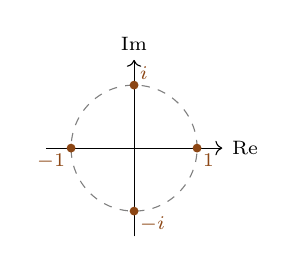
\begin{tikzpicture}[scale=0.8]
        \draw[->] (-1.4,0) -- (1.4,0) node[right]{\scriptsize Re};
        \draw[->] (0,-1.4) -- (0,1.4) node[above]{\scriptsize Im};
        \draw[gray, dashed] (0,0) circle (1);
        \fill[mAccent] (1,0) circle (2pt) node[below right=-2pt]{\scriptsize $1$};
        \fill[mAccent] (0,1) circle (2pt) node[above right=-2pt]{\scriptsize $i$};
        \fill[mAccent] (-1,0) circle (2pt) node[below left=-2pt]{\scriptsize $-1$};
        \fill[mAccent] (0,-1) circle (2pt) node[below right=-2pt]{\scriptsize $-i$};
      \end{tikzpicture}
    \end{column}
  \end{columns}

  \note{
    Example "d" takes integer powers of the imaginary unit "i". The
    sequence runs through the four values shown on the slide, "i",
    negative 1, negative "i", and 1, and then repeats forever. It
    never settles, so it diverges. But it only ever visits four
    distinct points, so its range is finite. And since those four
    points lie on the unit circle, the sequence is bounded.
  }
\end{frame}

% --- Example (e) ---
\begin{frame}{Example 3.1 (e): Constant Sequence $s_n = 1$}
  \begin{exblock}{Sequence: $s_n = 1$ for all $n$}
    \[
      1,\; 1,\; 1,\; 1,\; 1,\; \dots
    \]
    \begin{itemize}
      \item Converges: \; $\displaystyle\lim_{n\to\infty} s_n = 1$
      \item Range: \; finite --- $\{1\}$
      \item Bounded
    \end{itemize}
  \end{exblock}

  \vspace{0.4em}
  \textbf{Lesson:} The range of a convergent sequence may still be finite.

  \note{
    Finally, example "e" is the constant sequence that takes the value
    1 everywhere. Trivially it converges to 1, its range is just the
    single point 1, and it is bounded. The takeaway from examples "d"
    and "e" is that a finite range alone tells us nothing about
    convergence: the constant sequence "e" converges, while the cyclic
    sequence "d" diverges, even though both have finite range.
  }
\end{frame}

% =============================================================================
\section{Properties of Convergent Sequences (Theorem 3.2)}
% =============================================================================

% --- Theorem 3.2 Statement: Build 1/4 ---
\begin{frame}{Theorem 3.2: Four Properties of Convergent Sequences}
  Let $\{p_n\}$ be a sequence in a metric space $X$.
  \begin{thmblock}{Theorem 3.2}
    \begin{enumerate}
      \item[(a)] $p_n \to p$ $\iff$ every neighborhood of $p$ contains $p_n$ for all but finitely many $n$.
    \end{enumerate}
  \end{thmblock}

  \note{
    Theorem 3.2 collects four fundamental properties of convergent
    sequences. We will build the statement up one part at a time. Part
    "a" is a rephrasing of the definition in topological language. It
    says convergence to "p" is equivalent to the condition that every
    neighborhood of "p", no matter how small, contains all but finitely
    many terms of the sequence. This is the same idea as the epsilon-
    "N" definition, but phrased without mentioning epsilon at all.
  }
\end{frame}

% --- Theorem 3.2 Statement: Build 2/4 ---
\begin{frame}{Theorem 3.2: Four Properties of Convergent Sequences}
  Let $\{p_n\}$ be a sequence in a metric space $X$.
  \begin{thmblock}{Theorem 3.2}
    \begin{enumerate}
      \item[(a)] $p_n \to p$ $\iff$ every neighborhood of $p$ contains $p_n$ for all but finitely many $n$.
      \item[(b)] If $p_n \to p$ and $p_n \to p'$, then $p = p'$. \; (\alert{uniqueness})
    \end{enumerate}
  \end{thmblock}

  \note{
    Part "b" is the uniqueness statement: a sequence cannot converge to
    two different limits. If two candidate limits "p" and "p" prime
    both satisfy the definition, they must be the same point. This is
    what justifies calling the limit the limit rather than a limit.
  }
\end{frame}

% --- Theorem 3.2 Statement: Build 3/4 ---
\begin{frame}{Theorem 3.2: Four Properties of Convergent Sequences}
  Let $\{p_n\}$ be a sequence in a metric space $X$.
  \begin{thmblock}{Theorem 3.2}
    \begin{enumerate}
      \item[(a)] $p_n \to p$ $\iff$ every neighborhood of $p$ contains $p_n$ for all but finitely many $n$.
      \item[(b)] If $p_n \to p$ and $p_n \to p'$, then $p = p'$. \; (\alert{uniqueness})
      \item[(c)] $\{p_n\}$ convergent $\;\Longrightarrow\;$ $\{p_n\}$ \alert{bounded}.
    \end{enumerate}
  \end{thmblock}

  \note{
    Part "c" says that every convergent sequence is bounded. Intuitively,
    if the tail of the sequence is trapped near the limit, it cannot
    run off, and the initial segment has only finitely many terms, so
    altogether the sequence stays inside some bounded region.
  }
\end{frame}

% --- Theorem 3.2 Statement: Build 4/4 ---
\begin{frame}{Theorem 3.2: Four Properties of Convergent Sequences}
  Let $\{p_n\}$ be a sequence in a metric space $X$.
  \begin{thmblock}{Theorem 3.2}
    \begin{enumerate}
      \item[(a)] $p_n \to p$ $\iff$ every neighborhood of $p$ contains $p_n$ for all but finitely many $n$.
      \item[(b)] If $p_n \to p$ and $p_n \to p'$, then $p = p'$. \; (\alert{uniqueness})
      \item[(c)] $\{p_n\}$ convergent $\;\Longrightarrow\;$ $\{p_n\}$ \alert{bounded}.
      \item[(d)] $E \subset X$, $p$ a limit point of $E$ $\;\Longrightarrow\;$ $\exists\, \{p_n\} \subset E$ with $p_n \to p$.
    \end{enumerate}
  \end{thmblock}

  \note{
    Part "d" is the bridge between topology and sequences. If a point
    "p" is a limit point of a set "E", meaning every neighborhood of
    "p" contains a point of "E" other than "p" itself, then we can
    actually choose a sequence of points in "E" that converges to "p".
    This is what lets us translate limit-point statements into sequence
    statements, and vice versa. We now prove all four parts.
  }
\end{frame}

% --- Proof 3.2(a): Build 1/2 ---
\begin{frame}{Proof of 3.2(a): Forward Direction}
  \begin{proofblock}{$\Rightarrow$ direction}
    Suppose $p_n \to p$ and let $V$ be a neighborhood of $p$. \\
    Then $\exists\,\varepsilon > 0$ such that $d(q,p) < \varepsilon \Rightarrow q \in V$.

    \vspace{0.3em}
    By definition, $\exists\, N$ with
    \[
      n \geq N \;\Longrightarrow\; d(p_n, p) < \varepsilon \;\Longrightarrow\; p_n \in V.
    \]
    So $V$ contains $p_n$ for all $n \geq N$: all but finitely many.
  \end{proofblock}

  \note{
    We prove part "a" by proving both directions of the biconditional.
    First the forward direction: assume "p" sub "n" converges to "p",
    and let "V" be any neighborhood of "p". Every neighborhood contains
    a ball around "p", so there is some positive epsilon such that any
    point within epsilon of "p" lies in "V". The definition of
    convergence then gives us an index "N" beyond which the sequence
    stays within epsilon of "p", hence inside "V". That leaves at most
    the first "N" minus 1 terms outside "V": finitely many.
  }
\end{frame}

% --- Proof 3.2(a): Build 2/2 ---
\begin{frame}{Proof of 3.2(a): Converse}
  \begin{proofblock}{$\Leftarrow$ direction}
    Suppose every neighborhood of $p$ contains all but finitely many of the $p_n$.

    \vspace{0.3em}
    Fix $\varepsilon > 0$. Set $V = \{q \in X : d(p,q) < \varepsilon\}$ (the $\varepsilon$-ball).

    \vspace{0.3em}
    By assumption, $\exists\, N$ with $p_n \in V$ for $n \geq N$.

    \vspace{0.3em}
    Hence $d(p_n, p) < \varepsilon$ for $n \geq N$, so $p_n \to p$. \quad $\blacksquare$
  \end{proofblock}

  \note{
    For the converse, assume the neighborhood condition holds, and we
    must derive convergence. Fix any positive epsilon, and take "V" to
    be the open epsilon-ball around "p". Since "V" is a neighborhood of
    "p", by hypothesis all but finitely many terms lie inside "V",
    which means there is an index "N" such that every "p" sub "n" with
    "n" at least "N" lies within epsilon of "p". That is exactly the
    definition of convergence, so "p" sub "n" converges to "p". Part
    "a" is done.
  }
\end{frame}

% --- Proof 3.2(b): Build 1/2 ---
\begin{frame}{Proof of 3.2(b): Uniqueness --- Setup}
  \begin{proofblock}{Setup}
    Suppose $p_n \to p$ and $p_n \to p'$. Fix $\varepsilon > 0$.

    \vspace{0.3em}
    Pick $N, N'$ so that
    \[
      n \geq N \;\Longrightarrow\; d(p_n, p) < \tfrac{\varepsilon}{2},
    \]
    \[
      n \geq N' \;\Longrightarrow\; d(p_n, p') < \tfrac{\varepsilon}{2}.
    \]
  \end{proofblock}

  \textbf{Strategy:} use the triangle inequality to bound $d(p, p')$ by $\varepsilon$.

  \note{
    For part "b", assume the sequence has two candidate limits "p" and
    "p" prime. We want to show these points must coincide. Fix any
    positive epsilon. By the definition of convergence applied to each
    candidate, we can find an index "N" past which every term is
    within epsilon over 2 of "p", and another index "N" prime past
    which every term is within epsilon over 2 of "p" prime. The
    strategy is to triangulate: use a late term "p" sub "n" as a
    stepping stone to bound the distance from "p" to "p" prime.
  }
\end{frame}

% --- Proof 3.2(b): Build 2/2 ---
\begin{frame}{Proof of 3.2(b): Uniqueness --- Triangle Inequality}
  \begin{proofblock}{Triangle inequality}
    Let $n \geq \max(N, N')$. Then
    \[
      d(p, p') \;\leq\; d(p, p_n) + d(p_n, p') \;<\; \tfrac{\varepsilon}{2} + \tfrac{\varepsilon}{2} = \varepsilon.
    \]
  \end{proofblock}

  \vspace{0.3em}
  \begin{proofblock}{Conclusion}
    $d(p, p') < \varepsilon$ for \alert{every} $\varepsilon > 0$ \;$\Longrightarrow$\; $d(p, p') = 0$
    \;$\Longrightarrow$\; $\boxed{p = p'.}$ \quad $\blacksquare$
  \end{proofblock}

  \note{
    Pick any "n" past both thresholds. By the triangle inequality, the
    distance from "p" to "p" prime is at most the distance from "p" to
    "p" sub "n" plus the distance from "p" sub "n" to "p" prime, which
    is less than epsilon over 2 plus epsilon over 2, that is, epsilon.
    Since epsilon was arbitrary, the distance from "p" to "p" prime is
    less than every positive number, so it must be 0. In a metric
    space, distance 0 means equality, so "p" equals "p" prime. The
    limit is unique.
  }
\end{frame}

% --- Proof 3.2(c): Build 1/2 ---
\begin{frame}{Proof of 3.2(c): Convergent $\Rightarrow$ Bounded --- Setup}
  \begin{proofblock}{Setup}
    Suppose $p_n \to p$. Take $\varepsilon = 1$: $\exists\, N$ with
    \[
      n > N \;\Longrightarrow\; d(p_n, p) < 1.
    \]
    So the \emph{tail} $p_{N+1}, p_{N+2}, \dots$ fits in the unit ball around $p$.
  \end{proofblock}

  What about the \alert{initial segment} $p_1, \dots, p_N$? Only finitely many points.

  \note{
    Part "c": a convergent sequence is bounded. Take epsilon equal to
    1 in the definition to get an index "N" such that every term past
    "N" is within distance 1 of the limit "p". That handles the tail
    of the sequence. The initial segment, consisting of "p" sub 1
    through "p" sub "N", has only finitely many terms, and finitely
    many points always fit inside some ball. We combine these two
    observations on the next slide.
  }
\end{frame}

% --- Proof 3.2(c): Build 2/2 ---
\begin{frame}{Proof of 3.2(c): Convergent $\Rightarrow$ Bounded --- Conclusion}
  \begin{columns}[T]
    \begin{column}{0.58\textwidth}
      \begin{proofblock}{Bounded radius}
        Define
        \[
          r = \max\,\{\,1,\; d(p_1, p),\; \dots,\; d(p_N, p)\,\}.
        \]
        Then $d(p_n, p) \leq r$ for \alert{every} $n$.
      \end{proofblock}

      \vspace{0.3em}
      \begin{proofblock}{Conclusion}
        $\{p_n\}$ sits inside the closed ball of radius $r$ around $p$.
        \;$\blacksquare$
      \end{proofblock}
    \end{column}
    \begin{column}{0.38\textwidth}
      \centering
      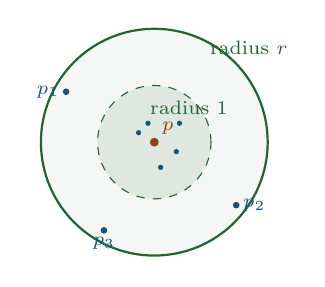
\begin{tikzpicture}[scale=0.8]
        % Outer ball of radius r
        \fill[proofcolor!5] (0,0) circle (1.8);
        \draw[proofcolor, thick] (0,0) circle (1.8);
        \node[proofcolor] at (1.5,1.5) {\scriptsize radius $r$};
        % Inner unit ball
        \fill[proofcolor!15] (0,0) circle (0.9);
        \draw[proofcolor, dashed] (0,0) circle (0.9);
        \node[proofcolor] at (0.55,0.55) {\scriptsize radius $1$};
        % p
        \fill[mAccent] (0,0) circle (2pt) node[above right=-1pt]{\scriptsize $p$};
        % Initial segment (outside unit, inside r)
        \fill[defcolor] (-1.4,0.8) circle (1.5pt) node[left=-1pt]{\scriptsize $p_1$};
        \fill[defcolor] (1.3,-1.0) circle (1.5pt) node[right=-1pt]{\scriptsize $p_2$};
        \fill[defcolor] (-0.8,-1.4) circle (1.5pt) node[below=-1pt]{\scriptsize $p_3$};
        % Tail (inside unit)
        \fill[defcolor] (0.4,0.3) circle (1.2pt);
        \fill[defcolor] (-0.25,0.15) circle (1.2pt);
        \fill[defcolor] (0.1,-0.4) circle (1.2pt);
        \fill[defcolor] (0.35,-0.15) circle (1.2pt);
        \fill[defcolor] (-0.1,0.3) circle (1.2pt);
      \end{tikzpicture}
    \end{column}
  \end{columns}

  \note{
    Define "r" to be the maximum of 1 and the "N" distances from the
    early terms to "p". The picture shows the two nested balls: the
    inner dashed ball of radius 1 traps the tail, because from index
    "N" onward every term is within 1 of "p". The outer solid ball of
    radius "r" additionally covers the initial segment "p" sub 1
    through "p" sub "N", because "r" is at least as large as each of
    those distances. Together, the entire sequence sits inside the
    outer ball, so it is bounded.
  }
\end{frame}

% --- Proof 3.2(d): Build 1/2 ---
\begin{frame}{Proof of 3.2(d): Limit Point $\Rightarrow$ Sequential Limit}
  \begin{columns}[T]
    \begin{column}{0.55\textwidth}
      \begin{proofblock}{Construction}
        $p$ is a limit point of $E$: every neighborhood of $p$ meets $E \setminus \{p\}$.

        \vspace{0.3em}
        For each $n = 1, 2, 3, \dots$ the ball $B(p, 1/n)$ meets $E$.

        \vspace{0.3em}
        Pick $p_n \in E$ with
        \[
          d(p_n, p) < \frac{1}{n}.
        \]
      \end{proofblock}
    \end{column}
    \begin{column}{0.42\textwidth}
      \centering
      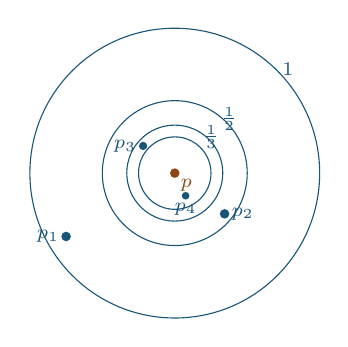
\begin{tikzpicture}[scale=1.15]
        % Nested balls of radius 1, 1/2, 1/3, 1/4
        \draw[defcolor, thin] (0,0) circle (1.6);
        \node[defcolor] at (1.25,1.15) {\scriptsize $1$};
        \draw[defcolor, thin] (0,0) circle (0.8);
        \node[defcolor] at (0.6,0.6) {\scriptsize $\tfrac{1}{2}$};
        \draw[defcolor, thin] (0,0) circle (0.53);
        \node[defcolor] at (0.4,0.4) {\scriptsize $\tfrac{1}{3}$};
        \draw[defcolor, thin] (0,0) circle (0.4);
        % p at center
        \fill[mAccent] (0,0) circle (1.5pt) node[below right=-2pt]{\scriptsize $p$};
        % p_1 inside radius 1 ball (but outside 1/2)
        \fill[defcolor] (-1.2,-0.7) circle (1.5pt) node[left=-1pt]{\scriptsize $p_1$};
        % p_2 inside 1/2 (outside 1/3)
        \fill[defcolor] (0.55,-0.45) circle (1.5pt) node[right=-1pt]{\scriptsize $p_2$};
        % p_3 inside 1/3 (outside 1/4)
        \fill[defcolor] (-0.35,0.3) circle (1.3pt) node[left=-1pt]{\scriptsize $p_3$};
        % p_4 inside 1/4
        \fill[defcolor] (0.12,-0.25) circle (1.2pt) node[below=-1pt]{\scriptsize $p_4$};
      \end{tikzpicture}
    \end{column}
  \end{columns}

  \note{
    Part "d": if "p" is a limit point of a set "E", we construct an
    actual sequence in "E" converging to "p". The picture on the right
    shows the idea: we draw nested balls around "p" with shrinking
    radii 1, one-half, one-third, and so on. By the definition of
    limit point, each ball contains a point of "E" other than "p",
    and we name that point "p" sub "n". The points march steadily
    toward "p" because their distances are forced below 1 over "n".
  }
\end{frame}

% --- Proof 3.2(d): Build 2/2 ---
\begin{frame}{Proof of 3.2(d): Verifying Convergence}
  \begin{proofblock}{Verify $p_n \to p$}
    Given $\varepsilon > 0$, by the Archimedean property choose $N$ with $N \varepsilon > 1$.

    \vspace{0.3em}
    For $n > N$:
    \[
      d(p_n, p) \;<\; \frac{1}{n} \;<\; \frac{1}{N} \;<\; \varepsilon.
    \]
    Hence $p_n \to p$. \quad $\blacksquare$
  \end{proofblock}

  \vspace{0.3em}
  \textbf{Consequence:} topology meets sequences --- limit points \emph{are} sequential limits from within $E$.

  \note{
    Now we verify convergence. Given any positive epsilon, use the
    Archimedean property of the reals to pick "N" with "N" times
    epsilon greater than 1, equivalently 1 over "N" less than epsilon.
    For any "n" beyond "N", the distance from "p" sub "n" to "p" is
    less than 1 over "n", which is less than 1 over "N", which is
    less than epsilon. So the sequence converges to "p". The
    consequence is that limit points of "E" are exactly the points
    that can be approached by sequences in "E". This is a crucial
    bridge we will use repeatedly.
  }
\end{frame}

% =============================================================================
\section{Arithmetic of Limits (Theorem 3.3)}
% =============================================================================

% --- Motivation ---
\begin{frame}{From Metric Spaces to Complex Sequences}
  \begin{remblock}{Context}
    Theorem 3.2 used only the metric $d$. Now we add \alert{algebraic structure}:
  \end{remblock}

  \vspace{0.4em}
  Complex sequences $\{s_n\}, \{t_n\} \subset \mathbb{C}$ can be \emph{added},
  \emph{multiplied}, \emph{divided}.

  \vspace{0.4em}
  \textbf{Question:} Do limits respect these operations?

  \vspace{0.4em}
  \alert{Yes} --- and the proofs are classical $\varepsilon$-style estimates.

  \note{
    Up to now we have only used the distance function "d". Metric
    spaces do not in general come with an algebra, but when the points
    are complex numbers we can add, multiply, and divide. The natural
    question is whether these operations play nicely with limits. If
    "s" sub "n" converges to "s" and "t" sub "n" converges to "t",
    does the sum "s" sub "n" plus "t" sub "n" converge to "s" plus "t"?
    The answer, as expected, is yes, and Theorem 3.3 makes this
    precise. Each proof is a short epsilon estimate.
  }
\end{frame}

% --- Theorem 3.3 Statement: Build 1/4 ---
\begin{frame}{Theorem 3.3: Arithmetic of Limits}
  Suppose $s_n \to s$ and $t_n \to t$ in $\mathbb{C}$. Then:
  \begin{thmblock}{Theorem 3.3}
    \begin{enumerate}
      \item[(a)] $\displaystyle\lim_{n\to\infty} (s_n + t_n) = s + t$
    \end{enumerate}
  \end{thmblock}

  \note{
    Part "a" says the limit of a sum is the sum of the limits. We will
    prove this using the same triangle-inequality trick as in the
    uniqueness proof, splitting an epsilon into two halves and bounding
    each piece separately.
  }
\end{frame}

% --- Theorem 3.3 Statement: Build 2/4 ---
\begin{frame}{Theorem 3.3: Arithmetic of Limits}
  Suppose $s_n \to s$ and $t_n \to t$ in $\mathbb{C}$. Then:
  \begin{thmblock}{Theorem 3.3}
    \begin{enumerate}
      \item[(a)] $\displaystyle\lim_{n\to\infty} (s_n + t_n) = s + t$
      \item[(b)] For any $c \in \mathbb{C}$: \; $\displaystyle\lim_{n\to\infty} cs_n = cs$, \; $\displaystyle\lim_{n\to\infty} (c + s_n) = c + s$
    \end{enumerate}
  \end{thmblock}

  \note{
    Part "b" handles scalar multiples and constants added to a
    convergent sequence. Since a constant "c" is trivially the limit
    of the constant sequence that takes value "c" everywhere, part "b"
    really just repackages part "a" together with the product rule in
    part "c", and the book describes the proof of "b" as trivial.
  }
\end{frame}

% --- Theorem 3.3 Statement: Build 3/4 ---
\begin{frame}{Theorem 3.3: Arithmetic of Limits}
  Suppose $s_n \to s$ and $t_n \to t$ in $\mathbb{C}$. Then:
  \begin{thmblock}{Theorem 3.3}
    \begin{enumerate}
      \item[(a)] $\displaystyle\lim_{n\to\infty} (s_n + t_n) = s + t$
      \item[(b)] For any $c \in \mathbb{C}$: \; $\displaystyle\lim_{n\to\infty} cs_n = cs$, \; $\displaystyle\lim_{n\to\infty} (c + s_n) = c + s$
      \item[(c)] $\displaystyle\lim_{n\to\infty} s_n t_n = st$
    \end{enumerate}
  \end{thmblock}

  \note{
    Part "c" is the product rule for limits, and it is the most
    interesting of the four. Its proof uses a clever algebraic
    identity that rewrites the difference "s" sub "n" times "t" sub
    "n" minus "s" "t" as three pieces, each of which we can control
    separately. We will see this shortly.
  }
\end{frame}

% --- Theorem 3.3 Statement: Build 4/4 ---
\begin{frame}{Theorem 3.3: Arithmetic of Limits}
  Suppose $s_n \to s$ and $t_n \to t$ in $\mathbb{C}$. Then:
  \begin{thmblock}{Theorem 3.3}
    \begin{enumerate}
      \item[(a)] $\displaystyle\lim_{n\to\infty} (s_n + t_n) = s + t$
      \item[(b)] For any $c \in \mathbb{C}$: \; $\displaystyle\lim_{n\to\infty} cs_n = cs$, \; $\displaystyle\lim_{n\to\infty} (c + s_n) = c + s$
      \item[(c)] $\displaystyle\lim_{n\to\infty} s_n t_n = st$
      \item[(d)] $\displaystyle\lim_{n\to\infty} \frac{1}{s_n} = \frac{1}{s}$, \; provided $s_n \neq 0$ and $s \neq 0$.
    \end{enumerate}
  \end{thmblock}

  \note{
    Part "d" is the reciprocal rule. We need the extra assumption that
    no term of the sequence is 0 and that the limit "s" itself is not
    0, otherwise 1 over "s" would not be defined. Once we have "d" and
    "c", the quotient rule follows by writing a ratio as a product
    times a reciprocal. We now turn to the proofs.
  }
\end{frame}

% --- Proof 3.3(a) ---
\begin{frame}{Proof of 3.3(a): Sum}
  \begin{proofblock}{The split-epsilon trick}
    Given $\varepsilon > 0$, pick $N_1, N_2$ so that
    \[
      n \geq N_1 \Rightarrow |s_n - s| < \tfrac{\varepsilon}{2}, \quad
      n \geq N_2 \Rightarrow |t_n - t| < \tfrac{\varepsilon}{2}.
    \]
    For $n \geq N = \max(N_1, N_2)$:
    \[
      |(s_n + t_n) - (s + t)| \leq |s_n - s| + |t_n - t| < \tfrac{\varepsilon}{2} + \tfrac{\varepsilon}{2} = \varepsilon.
    \]
  \end{proofblock}

  \vspace{0.3em}
  $\boxed{s_n + t_n \;\to\; s + t.}$ \quad $\blacksquare$

  \note{
    The proof of part "a" uses the split-epsilon trick. Given any
    positive epsilon, the convergence of "s" sub "n" to "s" gives an
    index "N" sub 1 past which the distance from "s" sub "n" to "s"
    is less than epsilon over 2; similarly for "t" sub "n" and "t".
    Past the maximum of the two indices, both bounds hold at once.
    The triangle inequality then bounds the deviation of the sum by
    epsilon over 2 plus epsilon over 2, that is, epsilon, which is
    exactly what convergence of the sum requires.
  }
\end{frame}

% --- Remark on 3.3(b) ---
\begin{frame}{Note on 3.3(b): Scalar and Constant}
  \begin{remblock}{Why 3.3(b) is ``trivial''}
    \textbf{Key observation:} the constant sequence $t_n := c$ converges to $c$
    (every term equals the limit, so the distance is always $0$).

    \vspace{0.4em}
    $\displaystyle\lim (c + s_n) = c + s$: \;
    apply (a) to $s_n$ and the constant sequence $t_n := c$.

    \vspace{0.2em}
    $\displaystyle\lim c \, s_n = c \, s$: \;
    apply (c) to $s_n$ and the constant sequence $t_n := c$.
  \end{remblock}

  \note{
    Part "b" is a quick corollary of parts "a" and "c" once we make one
    key observation: the constant sequence whose every term is "c"
    trivially converges to "c", because the distance from each term to
    the limit is always zero. Given that, adding "c" to "s" sub "n" is
    just a sum of two convergent sequences, which is covered by part
    "a"; and multiplying "s" sub "n" by "c" is a product of two
    convergent sequences, which is covered by part "c". The book calls
    the proof of part "b" trivial for exactly these reasons.
  }
\end{frame}

% --- Proof 3.3(c): Build 1/3 ---
\begin{frame}{Proof of 3.3(c): Product --- The Key Identity}
  \begin{proofblock}{Algebraic identity}
    \begin{equation}
      s_n t_n - s t = (s_n - s)(t_n - t) + s(t_n - t) + t(s_n - s). \tag{1}
    \end{equation}
  \end{proofblock}

  \vspace{0.3em}
  \textbf{Idea:} each of the three pieces on the right can be driven to $0$.
  \begin{itemize}
    \item $(s_n - s)(t_n - t)$ is \alert{quadratically small}.
    \item $s(t_n - t)$ and $t(s_n - s)$ are \alert{linearly small}.
  \end{itemize}

  \note{
    Part "c" is the one with a genuine trick. The identity on the
    slide rewrites the difference between "s" sub "n" times "t" sub
    "n" and the target product "s" "t" as a sum of three pieces. The
    first piece is a product of two small quantities and will be
    quadratically small. The other two pieces are each a fixed
    constant times a small quantity and will be linearly small. Once
    we can make each piece small, their sum is small, and that
    establishes the product rule.
  }
\end{frame}

% --- Proof 3.3(c): Build 2/3 ---
\begin{frame}{Proof of 3.3(c): Controlling the Quadratic Piece}
  \begin{proofblock}{First piece $\to 0$}
    Given $\varepsilon > 0$, pick $N_1, N_2$ so that
    \[
      n \geq N_1 \Rightarrow |s_n - s| < \sqrt{\varepsilon}, \qquad
      n \geq N_2 \Rightarrow |t_n - t| < \sqrt{\varepsilon}.
    \]
    For $n \geq \max(N_1, N_2)$:
    \[
      |(s_n - s)(t_n - t)| < \sqrt{\varepsilon} \cdot \sqrt{\varepsilon} = \varepsilon.
    \]
    Therefore $\displaystyle\lim_{n\to\infty} (s_n - s)(t_n - t) = 0$.
  \end{proofblock}

  \note{
    Let us drive the first piece to zero. Given epsilon, pick indices
    beyond which the distance from "s" sub "n" to "s" is less than the
    square root of epsilon, and similarly for "t" sub "n" to "t".
    Multiplying the two bounds, the absolute value of the product is
    less than epsilon. Since epsilon was arbitrary, this first piece
    tends to 0. The key observation is that when you multiply two
    small numbers, the product is much smaller than either factor
    alone.
  }
\end{frame}

% --- Proof 3.3(c): Build 3/3 ---
\begin{frame}{Proof of 3.3(c): Assembling the Product Rule}
  \begin{proofblock}{Assemble (1)}
    Looking at identity (1): \; $s_n t_n - st$ is a sum of three terms.
    \begin{itemize}
      \item $(s_n - s)(t_n - t) \to 0$ \; (just shown)
      \item $s(t_n - t) \to s \cdot 0 = 0$ \; (by 3.3(b))
      \item $t(s_n - s) \to t \cdot 0 = 0$ \; (by 3.3(b))
    \end{itemize}
    By 3.3(a), the sum of three null sequences is null:
    \[
      \lim_{n\to\infty}(s_n t_n - st) = 0 \;\Longrightarrow\; \boxed{s_n t_n \to s t.} \quad \blacksquare
    \]
  \end{proofblock}

  \note{
    Now we apply the parts of the theorem already proved. The second
    piece, "s" times the difference "t" sub "n" minus "t", goes to
    zero by part "b", scalar rule. The third piece similarly goes to
    zero. So all three pieces of identity 1 tend to zero. By part "a",
    the sum of three sequences that tend to zero also tends to zero.
    Hence "s" sub "n" times "t" sub "n" minus "s" "t" tends to zero,
    which is the product rule.
  }
\end{frame}

% --- Proof 3.3(d): Build 1/2 ---
\begin{frame}{Proof of 3.3(d): Reciprocal --- Bounding Away from 0}
  \begin{proofblock}{Step 1 --- Keep $|s_n|$ away from $0$}
    Since $s \neq 0$, apply convergence with $\tfrac{1}{2}|s|$:
    \[
      \exists\, m \text{ with } n \geq m \Rightarrow |s_n - s| < \tfrac{1}{2}|s|.
    \]
    Reverse triangle inequality $\Rightarrow$
    \[
      |s_n| > \tfrac{1}{2}|s| \quad (n \geq m).
    \]
  \end{proofblock}

  Why this matters: $1/s_n$ only makes sense if $|s_n|$ stays away from $0$.

  \note{
    The reciprocal rule has an extra wrinkle. The quantity 1 over "s"
    sub "n" is sensitive to "s" sub "n" being close to 0, so we need
    to keep "s" sub "n" away from 0 in a quantitative way. Since "s"
    is not 0, its absolute value is a positive number. Apply
    convergence with tolerance one-half of the absolute value of "s"
    to get an index "m" past which "s" sub "n" is within this small
    tolerance of "s". By the reverse triangle inequality, that forces
    the absolute value of "s" sub "n" to be more than one-half of the
    absolute value of "s", safely away from 0.
  }
\end{frame}

% --- Proof 3.3(d): Build 2/2 ---
\begin{frame}{Proof of 3.3(d): Reciprocal --- The Estimate}
  \begin{proofblock}{Step 2 --- Estimate the reciprocal}
    Given $\varepsilon > 0$, pick $N > m$ so that
    \[
      n \geq N \Rightarrow |s_n - s| < \tfrac{1}{2}|s|^2 \varepsilon.
    \]
    Then for $n \geq N$:
    \[
      \left|\tfrac{1}{s_n} - \tfrac{1}{s}\right|
      = \left|\tfrac{s_n - s}{s_n s}\right|
      < \tfrac{2}{|s|^2}\,|s_n - s|
      < \varepsilon.
    \]
    So $\;\boxed{\dfrac{1}{s_n} \;\to\; \dfrac{1}{s}.}$ \quad $\blacksquare$
  \end{proofblock}

  \note{
    For step 2, pick an index "N" past "m" such that the distance
    from "s" sub "n" to "s" is less than one-half absolute value of
    "s" squared times epsilon. The algebra on the slide writes the
    difference between the two reciprocals as a single fraction,
    uses the lower bound on the absolute value of "s" sub "n" from
    step 1 to bound the denominator, and then uses the epsilon
    estimate on the numerator. The result is bounded by epsilon, so
    the reciprocal of "s" sub "n" converges to the reciprocal of "s".
  }
\end{frame}

% =============================================================================
\section{Convergence in $\mathbb{R}^k$ (Theorem 3.4)}
% =============================================================================

% --- Setup ---
\begin{frame}{Moving Up to $\mathbb{R}^k$}
  \begin{remblock}{From $\mathbb{C}$ to $\mathbb{R}^k$}
    A sequence in $\mathbb{R}^k$ is a sequence of \alert{vectors}
    $\mathbf{x}_n = (\alpha_{1,n}, \alpha_{2,n}, \dots, \alpha_{k,n})$.
  \end{remblock}

  \vspace{0.4em}
  \textbf{Natural question:} What is the relationship between
  \begin{itemize}
    \item convergence of the \emph{vector} sequence $\{\mathbf{x}_n\}$, and
    \item convergence of each \emph{coordinate} sequence $\{\alpha_{j,n}\}$?
  \end{itemize}

  \note{
    Theorem 3.4 lifts the arithmetic results to sequences in "R" to
    the "k". A sequence of vectors in "R" to the "k" is really "k"
    sequences of real numbers bundled together, one for each
    coordinate. The natural question is whether the vector sequence
    converges exactly when every coordinate sequence converges, and
    if so, whether the components of the limit are the individual
    coordinate limits.
  }
\end{frame}

% --- Theorem 3.4 Statement: Build 1/2 ---
\begin{frame}{Theorem 3.4: Componentwise Convergence}
  \begin{thmblock}{Theorem 3.4 (a)}
    Let $\mathbf{x}_n = (\alpha_{1,n}, \dots, \alpha_{k,n}) \in \mathbb{R}^k$. Then
    \[
      \mathbf{x}_n \to \mathbf{x} = (\alpha_1, \dots, \alpha_k)
      \;\;\iff\;\;
      \lim_{n\to\infty}\alpha_{j,n} = \alpha_j \; \text{ for } 1 \leq j \leq k.
    \]
  \end{thmblock}

  \vspace{0.3em}
  Vector convergence $\iff$ convergence in \alert{every} coordinate.

  \note{
    Part "a" gives the clean answer: convergence of vectors in "R" to
    the "k" is equivalent to convergence of each coordinate sequence,
    and the components of the limit vector are precisely the limits
    of the coordinate sequences. This is a biconditional statement,
    so we will prove both directions.
  }
\end{frame}

% --- Theorem 3.4 Statement: Build 2/2 ---
\begin{frame}{Theorem 3.4: Algebraic Operations in $\mathbb{R}^k$}
  \begin{thmblock}{Theorem 3.4 (b)}
    If $\mathbf{x}_n \to \mathbf{x}$, $\mathbf{y}_n \to \mathbf{y}$ in $\mathbb{R}^k$ and
    $\beta_n \to \beta$ in $\mathbb{R}$, then
    \[
      \mathbf{x}_n + \mathbf{y}_n \to \mathbf{x} + \mathbf{y},
    \]
    \[
      \mathbf{x}_n \cdot \mathbf{y}_n \to \mathbf{x} \cdot \mathbf{y},
    \]
    \[
      \beta_n \mathbf{x}_n \to \beta \mathbf{x}.
    \]
  \end{thmblock}

  \vspace{0.3em}
  Limits commute with sum, dot product, and scalar multiplication.

  \note{
    Part "b" says limits respect vector addition, the dot product,
    and scalar multiplication by a sequence of scalars. These are
    the natural vector operations one would want to apply. The proof
    of part "b" comes for free once we have part "a", since each
    operation can be analyzed coordinate by coordinate using the
    complex-sequence rules of Theorem 3.3. Let us prove part "a".
  }
\end{frame}

% --- Proof 3.4(a): Build 1/2 ---
\begin{frame}{Proof of 3.4(a): $\Rightarrow$ Direction}
  \begin{proofblock}{From vector convergence to coordinate convergence}
    Suppose $\mathbf{x}_n \to \mathbf{x}$ in $\mathbb{R}^k$. For each fixed $j$,
    a single squared term is at most the full sum of squares:
    \[
      |\alpha_{j,n} - \alpha_j|^2
      \;\leq\; \sum_{i=1}^{k} |\alpha_{i,n} - \alpha_i|^2
      \;=\; |\mathbf{x}_n - \mathbf{x}|^2.
    \]
    Taking square roots:
    \[
      |\alpha_{j,n} - \alpha_j| \;\leq\; |\mathbf{x}_n - \mathbf{x}|.
    \]

    \vspace{0.2em}
    So $|\mathbf{x}_n - \mathbf{x}| \to 0$ \;$\Longrightarrow$\; $|\alpha_{j,n} - \alpha_j| \to 0$
    for every $j$.
  \end{proofblock}

  \note{
    The forward direction of part "a" is the easier one. The key
    inequality says that a single coordinate deviation is at most the
    full Euclidean norm of the difference vector. To see why, look at
    the slide: the squared norm of "x" sub "n" minus "x" is by
    definition the sum over all coordinates of the squared deviations,
    and any single one of those squares is obviously at most the whole
    sum. Taking square roots gives the inequality we want. Then if the
    vector norm goes to 0, every coordinate deviation is squeezed down
    to 0 as well, which is exactly the convergence of each coordinate
    sequence.
  }
\end{frame}

% --- Proof 3.4(a): Build 2/2 ---
\begin{frame}{Proof of 3.4(a): $\Leftarrow$ Direction}
  \begin{proofblock}{From coordinate convergence to vector convergence}
    Suppose $\alpha_{j,n} \to \alpha_j$ for each $1 \leq j \leq k$.
    Given $\varepsilon > 0$, pick $N$ so that $n \geq N$ implies
    \[
      |\alpha_{j,n} - \alpha_j| < \frac{\varepsilon}{\sqrt{k}} \qquad (1 \leq j \leq k).
    \]
    Then
    \[
      |\mathbf{x}_n - \mathbf{x}| = \left\{ \sum_{j=1}^{k} |\alpha_{j,n} - \alpha_j|^2 \right\}^{1/2}
      < \sqrt{k \cdot \tfrac{\varepsilon^2}{k}} = \varepsilon.
    \]
    Hence $\mathbf{x}_n \to \mathbf{x}$. \quad $\blacksquare$
  \end{proofblock}

  \note{
    For the converse, assume every coordinate sequence converges to
    the corresponding coordinate of "x". Given epsilon, apply
    convergence to each coordinate with tolerance epsilon over square
    root of "k", picking a common index "N" that works for all of
    them. The Euclidean norm of the difference vector is then bounded
    by the square root of the sum of "k" squared quantities, each
    less than epsilon squared over "k". The sum is less than epsilon
    squared, so the norm is less than epsilon. That is exactly what
    convergence of the vector sequence requires.
  }
\end{frame}

% --- 3.4(b) corollary ---
\begin{frame}{Proof of 3.4(b): Operations Preserve Limits}
  \begin{proofblock}{By reduction to 3.3}
    Write $\mathbf{x}_n \cdot \mathbf{y}_n = \displaystyle\sum_{j=1}^{k} \alpha_{j,n} \beta_{j,n}$ where
    $\mathbf{y}_n = (\beta_{1,n}, \dots, \beta_{k,n})$.

    \vspace{0.3em}
    By 3.4(a), $\alpha_{j,n} \to \alpha_j$ and $\beta_{j,n} \to \beta_j$.

    \vspace{0.3em}
    By 3.3(a)+(c), each $\alpha_{j,n}\beta_{j,n} \to \alpha_j \beta_j$,
    and the sum of $k$ such terms tends to $\mathbf{x} \cdot \mathbf{y}$.

    \vspace{0.3em}
    Sum and scalar multiplication follow similarly. \quad $\blacksquare$
  \end{proofblock}

  \note{
    Part "b" is a corollary. The dot product of two vectors is a sum
    of "k" products of coordinates. By part "a" each coordinate
    sequence converges, and by the product rule and sum rule of
    Theorem 3.3, each coordinate product converges and the sum of
    "k" such converging sequences converges to the dot product of
    the two limit vectors. The sum and scalar-multiplication rules
    follow in the same way, coordinate by coordinate.
  }
\end{frame}

% =============================================================================
\section{Summary}
% =============================================================================

% --- Summary Build 1/5 ---
\begin{frame}{Summary}
  \textbf{Key takeaways from this section:}
  \begin{itemize}
    \item \alert{Definition 3.1}: $p_n \to p$ if $\forall\,\varepsilon > 0, \exists\, N$ with $n \geq N \Rightarrow d(p_n, p) < \varepsilon$.
  \end{itemize}

  \note{
    Let us review what we have learned. Definition 3.1 gave us the
    formal epsilon-"N" condition for convergence in a metric space:
    for every positive tolerance, eventually every term is within
    that tolerance of the limit.
  }
\end{frame}

% --- Summary Build 2/5 ---
\begin{frame}{Summary}
  \textbf{Key takeaways from this section:}
  \begin{itemize}
    \item \alert{Definition 3.1}: $p_n \to p$ if $\forall\,\varepsilon > 0, \exists\, N$ with $n \geq N \Rightarrow d(p_n, p) < \varepsilon$.
    \item \alert{Theorem 3.2}: neighborhood form, \emph{uniqueness}, bounded, limit-point bridge.
  \end{itemize}

  \note{
    Theorem 3.2 gave us the four basic properties of convergent
    sequences: a topological reformulation in terms of
    neighborhoods, uniqueness of the limit, boundedness of any
    convergent sequence, and the fundamental bridge that every limit
    point is a sequential limit.
  }
\end{frame}

% --- Summary Build 3/5 ---
\begin{frame}{Summary}
  \textbf{Key takeaways from this section:}
  \begin{itemize}
    \item \alert{Definition 3.1}: $p_n \to p$ if $\forall\,\varepsilon > 0, \exists\, N$ with $n \geq N \Rightarrow d(p_n, p) < \varepsilon$.
    \item \alert{Theorem 3.2}: neighborhood form, \emph{uniqueness}, bounded, limit-point bridge.
    \item \alert{Theorem 3.3}: limits of sums, products, and reciprocals for $\mathbb{C}$-sequences.
  \end{itemize}

  \note{
    Theorem 3.3 established the arithmetic of limits for complex
    sequences: limits respect sums, products, and reciprocals, with
    the reciprocal rule requiring the limit to be nonzero. The proofs
    were classical epsilon estimates, with the product rule relying
    on a clever algebraic identity that splits the difference into
    quadratically and linearly small pieces.
  }
\end{frame}

% --- Summary Build 4/5 ---
\begin{frame}{Summary}
  \textbf{Key takeaways from this section:}
  \begin{itemize}
    \item \alert{Definition 3.1}: $p_n \to p$ if $\forall\,\varepsilon > 0, \exists\, N$ with $n \geq N \Rightarrow d(p_n, p) < \varepsilon$.
    \item \alert{Theorem 3.2}: neighborhood form, \emph{uniqueness}, bounded, limit-point bridge.
    \item \alert{Theorem 3.3}: limits of sums, products, and reciprocals for $\mathbb{C}$-sequences.
    \item \alert{Theorem 3.4}: convergence in $\mathbb{R}^k$ is \emph{componentwise}, and operations commute with limits.
  \end{itemize}

  \note{
    Theorem 3.4 extended these results to "R" to the "k". Vector
    convergence is equivalent to simultaneous convergence of every
    coordinate, and vector addition, the dot product, and scalar
    multiplication all commute with limits. This reduces "R" to the
    "k" analysis to one-dimensional analysis, one coordinate at a
    time.
  }
\end{frame}

% --- Summary Build 5/5 ---
\begin{frame}{Summary}
  \textbf{Key takeaways from this section:}
  \begin{itemize}
    \item \alert{Definition 3.1}: $p_n \to p$ if $\forall\,\varepsilon > 0, \exists\, N$ with $n \geq N \Rightarrow d(p_n, p) < \varepsilon$.
    \item \alert{Theorem 3.2}: neighborhood form, \emph{uniqueness}, bounded, limit-point bridge.
    \item \alert{Theorem 3.3}: limits of sums, products, and reciprocals for $\mathbb{C}$-sequences.
    \item \alert{Theorem 3.4}: convergence in $\mathbb{R}^k$ is \emph{componentwise}, and operations commute with limits.
  \end{itemize}

  \vspace{0.6em}
  \textbf{Coming up next:} \emph{Subsequences} --- when subsequences converge, and
  the powerful notion of \emph{subsequential limits}.

  \note{
    In the next section we turn to subsequences. A subsequence is
    what you get by keeping only some of the terms of a sequence and
    preserving their order. We will see when passing to a subsequence
    preserves convergence, and we will discover that every bounded
    sequence in "R" to the "k", even if it fails to converge, has a
    convergent subsequence. See you there.
  }
\end{frame}

\end{document}
